\section{Pilot Experiment}
In this section, we introduce the pilot experiment we conducted prior to the large scale experiment. In general pilot experiments are a method to test feasibility and provide experience-based guidelines for follow up experiments. 
\subsection{Introduction}
The pilot experiment was conducted in the facilities of Systems Neuroscience and Neurotechnology Unit, particularly the Mindscan Lab, located at the HTW Saar (Technikum). The main goal of this experiment was to gather an initial set of authentic data while also testing the functionality of our data transmission routine and familiarizing ourselves with hardware and software behavior under experiment conditions. \\
The measurement was performed in a closed off laboratory environment with controlled temperature and illumination. Physiological signals were recorded using the Empatica E4, which was placed on the wrist of the non-dominant hand, and a laptop, serving as Processing Unit, that was placed approximately 1.5 meters away from the subject position.
We measured 2 subjects in this pilot experiment. They were bachelor level male students, studying at the HTW Saar aged between 26 and 30 years.

\subsection{Objectives}
\begin{itemize}
\item Test the procedure and the experimental design
\item Identify problems and optimization possibilities
\item Estimation of time and resource requirements
\item Inspect data quality
\end{itemize}
\subsection{Experimental Setup}
The experimental setup can be divided into two major components. The first component, is responsible for data acquisition and is comprised of the Empatica E4 and the Processing Unit. Whereas the second, handles the presentation of the experimental paradigm using a second Notebook in combination with a monitor.
During the experiment the subject is positioned in a chair in front of the monitor. The recording site is surrounded by movable walls serving as visual cover. Directly behind the cover, and to the side of the recording site, a desk has been placed to provide space for the Processing Unit, the operator, as well as any additional devices needed for the experiment. The distance between the E4, when worn by the subject, and the Processing Unit was approximately 1.5 meters.
%During the measurement the subjects were sitting in a chair, in an upright position, facing a monitor on the desk in front of them.
\subsection{Experimental Procedure}
In preparation of the experiment all participants were given a step-by-step explanation of the experimental procedure, to make sure they were in a relaxed and comfortable mood. After, the subjects had given their consent, they were asked to remove any electronic devices from their person and take a seat in the chair. Then, they were instructed to put on the Empatica E4. If necessary an operator would assist them. Once they were finished, the operator inspected the placement of the wristband in regards to the general fit, and sensor-skin contact. Prior to the start of the paradigm the participants were again reminded to be as relaxed as possible, make themselves comfortable, and avoid extensive movement. During the experiment the subjects were required to sit in front of the monitor and observe the paradigm, which was displayed on it, for a period of 5 minutes. 
\subsection{Paradigm}
The paradigm that was used in the pilot experiment, was comprised of a single picture showing a simple black cross-hair on a white background. The paradigm was created with PsychoPy, which was running on a Notebook, connected to the monitor. 
\subsection{Problem Oriented}
From the feedback we were given by the subjects, we were able to identify the following problems:
\begin{itemize}
\item The participants reported that the motive of the paradigm was causing them discomfort as the contrast between black and white was too extreme.
\item Both participants felt that the chair was not providing enough comfort due to missing armrests and height difference to the table. 
\end{itemize}
Further, we observed a slight offset in system time between the Processing Unit and the Notebook we used to run PsychoPy that could potentially raise issues in subsequent data analysis.

\subsection{Solution Oriented}
To address the aforementioned problems we altered the color scheme of our paradigm to provide a softer contrast (grey/white), exchanged the chair, and implemented a time synchronization routine in the experimental procedure.

\subsection{Results and Conclusion}
Because the results of our pilot experiment were overall positive we felt reassured to proceed to the main experiment with few alterations. We were able to successfully test the experimental procedure and the functionality of the setup. Further we were able to record quality data and gained valuable insight on the extent of the pre-processing needed to prepare the signals for feature extraction. We also gained a better understanding of the time-frame needed for the preparation, and the post-production of the experiment.

\section{Main Experiment}
In this section we present the main experiment of this thesis, which was conducted subsequently to our pilot experiment.
\subsection{Introduction}
 


All measurements were conducted within the facilities of Systems Neuroscience and Neurotechnology Unit, particularly the Green Lab, located at the University Hospital Saarland, and the Mindscan Lab, located at the HTW Saar (Technikum).
  
\subsection{Participants}
% talk about composition of subject group
In total 14 subjects, of which 7 were male and 7 female, participated in the experiment. Subject age ranged from 24 to 50 years, with an average of 29 years. At the day of the experiment all participants reported to be feeling well and capable of partaking in the experiment. 
\subsection{Methods}
In the following we will briefly discuss the methods we used in our experiment to elicit certain emotional states, as well as different degrees of mental workload.
\subsubsection{Stroop Test}
A color word test we used for a medium level of mental workload. This was confirmed by the subjective rating of the subjects, which on avg reported a difficulty of X on a scale of 1 to 10, with 1 being not stressed at all and 10 being completely stressed out (  state the results of difficulty rating stress level). The principle behind this test ... . Therefore it is used very often in studies involving attention and cognition??? (find sth to proof this)

We used a Stroop test featuring 11 different colors, resulting in a total of 220 trials the subjects had to work through. Although the color palette seems rather extensive when compared to the standard 3 color variation of the test, this was a conscious decision to guarantee a test time of at least 5 minutes while mitigating the monotony of the test. Each trial presented the subject with a colored word in the center of the screen and one possible answer to either side. The participants then had to choose the right answer based on the color of the word. Each decision was recorded via a key press on the keyboard. 

\subsubsection{7-Row}
We used this method to induce a high amount of stress causing a high workload in the subject. Again the subjective ratings confirmed the success of this method. Participants rated on avg a difficulty of X and a stress level of Y.

The test has the subjects count backwards from a certain integer in steps of 7, they have to do it aloud while the pace is given by the observed paradigm on the monitor. The operator monitors the process and intervenes when needed.. this means if one of the following situations occurred: 
- subject makes mistake - operator gives last correct value, asks to continue
- subject slows down - operator gives a warning and urges to increase the speed again
- subject shows deviant behavior such as increased movement - again operator corrects behavior

We used 7 row starting at 700 and used a blinking dot with changing color and increasing speed at certain time thresholds. If a subject completed the task before the five minute mark we would give them a new number between 1400 and 700 and let them continue.

\subsubsection{Visual Stimulation}
Visual stimulation using videos and pictures of certain motives is a commonly used method to elicit emotions. We used a collection of pictures from the IAPS.
We created to sets of pictures, each "displaying" one emotion. We chose positive valence/positive arousal, neutral valence/ positive arousal rated pictures i.e. positive or neutral pictures for eliciting a pleasant state and pictures that were rated negative valence/negative arousal, neutral valence/negative arousal i.e. negative motives to elicit an unpleasant state.
Set one for pleasant consisted of X pictures and set two for unpleasant consisted of Y pictures.
We can not show the chosen pictures due to infringement but we will give a list of descriptions in the appendix.
\subsection{Procedure}
One of the most important parts to this project was the collection of authentic data that could be used later on to develop a reliable classifier for our system. For that reason an experiment, specifically designed to elicit certain emotional and cognitive states in a subject, was conducted. The following section is focused on the procedure applied in this experiment.

The procedure was comprised of a total of five sessions. Every experiment was initiated with a short briefing session. Containing a short questionnaire, covering personal information of the participant as well as habits that may have a influence on the measurement. Further a series of questions, regarding their handedness, use and frequency of use of watches or other wearables was posed, to estimate the additional influence that may be caused by wearing the Empatica E4 wristband.
Concluding the first session, the participants were given a coarse outline of the experiment covering the structure and a basic description of their responsibilities.

The second session consisted of a baseline measurement used to log the participants form of the day and also to be able to account for environmental influences in the following processing steps. Before the start of the measurement the subject was placed on a chair in front of a monitor (24 inches, Resolution: 1080p) with a approximated distance of 1m. The Empatica E4 was then put on the wrist of the non-dominant hand and secured in a position that caused minimal light leakage to the PPG-sensor and provided optimal contact for the \gls{gsr} electrodes. After the participants were comfortable with the device a one minute test sequence was measured to verify the functionality of the system.
Consequently the paradigm was displayed on the monitor and the session was started. After reading the instructions, in which the subjects were asked to relax and remain still, and confirmation with the participant the measurement was initiated with a ten second countdown to give some additional time for preparation.
During the measurement the \gls{gsr}, \gls{bvp}, and temperature of the subject were measured for a duration of five minutes.
Afterwards, to conclude the second session, the participants had to give a subjective rating of their current mental state, regarding their stress level, ranging from 1 (completely relaxed) to 10 (stressed out).

The third session was comprised of three separate measurements, two cognitive tasks and a relaxation segment. As before a rating followed the recording. The ratings consisted of a subjective assessment by the subjects regarding their stress level. Additionally subjects had to rate the test difficulty on a scale from 1 (very easy) to 10 (very difficult) for both tasks. 
For the first measurement the subjects were instructed to count down aloud from 700 in steps of 7 while maintaining a certain pace. The counting rhythm was indicated by a flashing dot on the instruction screen, for a duration of five minutes. The dot's color and flashing frequency were altered during the experiment to further increase difficulty at the three and four minute mark. If the participants were to slow down or loose track an instructor would intervene to help.
The second task consisted of a Stroop-Word-Color test. The test featured 11 different colors, resulting in a total of 220 trials the subjects had to work through. Although the color palette seems rather extensive when compared to the standard 3 color variation of the test, this was a conscious decision to guarantee a test time of at least 5 minutes to mitigate monotony. Each trial presented the subject with a colored word in the center of the screen and one possible answer to either side. The participants then had to choose the right answer based on the color of the word. Each decision was recorded via a key press on the keyboard. 

%Wearing the device is as easy as wearing a watch.
%Wear the E4 with the case on top of your wrist. Wear it snugly, so that it does not move around,

%but not so tight that it is uncomfortable.
%Which side should you wear it on? Traditional recommendations are to record EDA on the nondominant
%side to minimize motion artifacts (e.g. a right-hander would wear it on their left wrist).
%However, recent studies show that the dominant side may have a much stronger EDA signal during
%certain kinds of stress. Also, neurological events (such as seizures) may elicit EDA on only one side.
%(For more information see: Picard, R. W., Fedor, S., & Ayzenberg Y., “Multiple Arousal Theory and Daily-
%Life Electrodermal Activity Asymmetry” Emotion Review, March 2015.). Depending on your purposes,
%you may want to measure on the right, left, or both wrists.
%The E4 button may be positioned on the same side as the thumb or on the other side – either
%orientation works fine.
%The EDA electrodes (under the snaps) should be on the inside of the wrist. You may optionally line
%them up with a finger, e.g. the third (ring) finger, but this is not required
%\begin{figure}[ht]
%	\centering
%  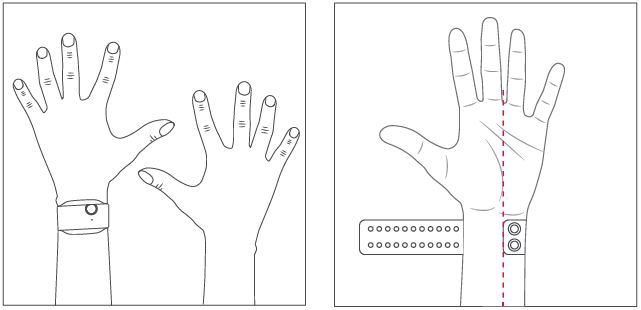
\includegraphics[width=0.33\textwidth]{../images/E4wearing.JPG}
%	\caption{A figure depicting the intended way the E4 wristband should be worn.}
%	\label{e4wearing}
%\end{figure}